% Hopefully this will be the final version of Problem statement.
\section{Problem Statement}

Data centers are large-scale computing infrastructures which consume huge amount of energy each year: a typical data center consumes as much energy as 25,000 households \cite{Dayarathna:2016ua}. Thus, reducing the energy consumption becomes the major concern of Cloud providers. 
In addition, data centers and computation powers support the modern Cloud computing industry, software industry and etc. Therefore, reducing the cost of data centers will lead to a reduction of cost of softwares which consequently be beneficial to most people who access the Internet on a daily basis.
Among several components that consume energy such as cooling system, physical machines (PMs) (e.g servers), and network devices, PMs accounts for 40\% and have a huge improvement space, since they are always in low utilization (e.g on average, from 10\% to 50\% of required resources) \cite{Barroso:2007jt,Shen:2015hm}. This low utilization of resource problem can be solved by fine granularity management of Cloud resources (e.g CPUs and RAMs) using a new virtualization technology: containers \cite{Felter:2015ki, He:2012im, Soltesz:2007cu} and a new service model: Container as a Service (CaaS) \cite{Piraghaj:2015uf}. CaaS is a mixture of traditional IaaS (Infrastructure as a Service) \cite{Mell:2011jj} and PaaS (Platform as a Service); it utilizes both containers and virtual machines (VMs) as the fundamental resource management units.
In CaaS, applications that were used to deployed in VMs (e.g in IaaS) are now deployed in containers. Container is an operating system (OS) level of virtualization; multiple containers can run on a VM and share OS. Therefore, server consolidation \cite{Varasteh:2015fu} can be applied in a joint of containers and VMs environment to achieve better energy reduction.


% (What is the problem? (variables, objectives))(Why important?)(What are the processes?) 

\begin{figure}
	\centering
	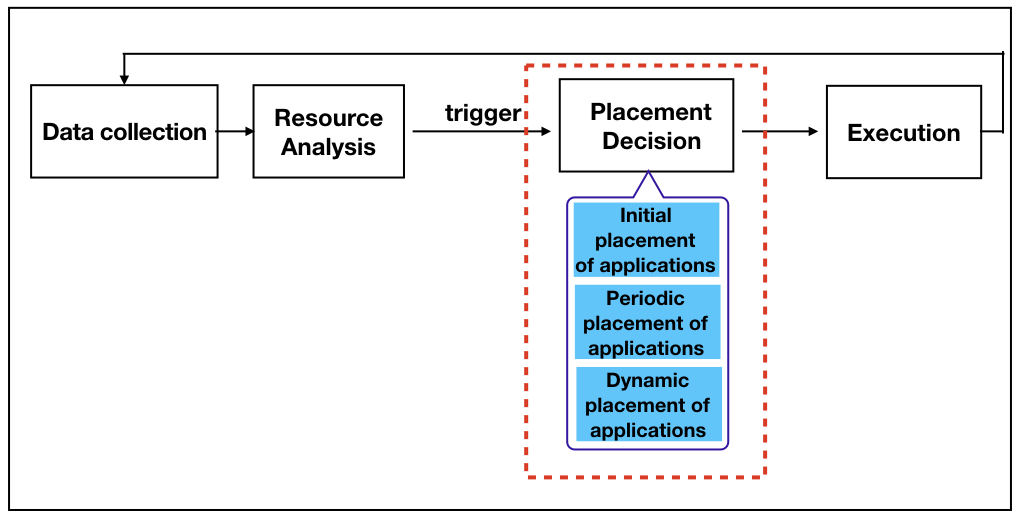
\includegraphics[width=0.7\textwidth]{pics/workflow_management.png}
	\caption{A workflow of resource management \cite{Mishra:2012kx}}
	\label{fig:workflow}
\end{figure}

Server consolidation is an important strategy in improving the utilization throughout the Cloud resource management processes as shown in Figure \ref{fig:workflow} including new application allocation \cite{Jennings:2015ht}, periodic optimization \cite{Mishra:2012kx}, overloading and under-loading adjustments \cite{Mishra:2012kx}. According to the characteristic of each process, server consolidation can be roughly classified into two categories: static problems \cite{Mishra:2012kx} and dynamic problems \cite{Beloglazov:2012bw}.
Accordingly, server consolidation approaches also have corresponding categories. Static approaches use historical average resource utilization data as input to map applications to PMs. Static consolidation normally involves large amount of applications and PMs, therefore, the optimization is quite time-consuming and often conducted in a off-line fashion. Periodic optimization belongs to this category. It takes a number of existing applications and re-allocate them into a number of PMs. 
Dynamic approaches take one application each time, allocates it into one of the PMs. The operation is conducted in an online fashion, therefore, it requires fast reaction. Overloading  and under-loading can be categories to dynamic consolidation problem \cite{Beloglazov:2013ht}. New application allocation can be seen as either static: allocate a batch of new applications, or dynamic: allocate a new application each time. In this proposal, we consider it as a static problem. 
% These three consolidation problems can be seen distinct optimization tasks which have a common goal: minimizing the energy consumption of a data center. 

Examples of static server consolidation are shown in the following in VM-based and container-based Cloud. In traditional VM-based Cloud, Server consolidation can be described as, given a number of Physical Machines (PMs) which can be represented as the resources(e.g CPU cores and RAM); a number of requests for fixed configurations of VMs (assume applications have been deployed in VMs), each configuration can also be represented as aforementioned resources; The objective is to allocate these requested VMs into a minimum number of PMs. The decision variable is the location of each requested VM. In container-based Cloud, instead of allocating requested VMs in PMs, a set of containers (assume applications have been deployed into containers) represented as resources is first allocated to a number of fixed type VMs, then, these VMs are allocated to PMs. The decision variables are the allocation of containers (upper level) and VMs (lower level). For the upper level of allocation, the objective is to maximize the utilization of resources (e.g a balanced utilization among several resources), while the lower level objective is to minimize the number of PMs.

Traditional VM-based server consolidation are modeled as bin-packing problems \cite{Mann:2015ua}. This is because VMs and PMs are naturally modeled as items and bins and server consolidation and bin-packing have the same optimization objective: minimize the number of bins/PMs. The complexity of bin-packing problem is NP-hard which means it is extreme time-consuming to find its optimal solution when the number of decision variables are large. Container-based server consolidation can be categorized as a bilevel optimization problem \cite{Colson:2007bu}. Bilevel problems are typically non-convex and strongly NP-hard \cite{Vicente:1994ie}. In this case, two levels are lower-level: Containers to VM and upper-level: VMs to PMs. These two levels optimization are connected through decision variables. In this case, two levels of optimization are both bin packing problems and they are cooperating \cite{Legillon:2012dd}.

Currently, most research focus on VM-based server consolidation and these methods can not be directly applied on container-based consolidation because of the different structure. Only few research focus on container-based server consolidation problem. One of the state-of-the-art research is from Piraghaj and et al \cite{Piraghaj:2015uf}. They first propose a VM-resizing technique that defines the types of VM based on analyzing the historical data from Google. Then they propose a two-step allocation: first allocate containers to VMs and then allocate VMs to PMs. Their major contribution is the method of defining types of VM. The allocation of containers does not optimize the energy consumption and the allocation of VMs are traditional First Fit algorithm. In addition, they propose a dynamic consolidation \cite{Piraghaj:2016bw} using a series simple heuristics such as Random Host Selection Algorithm or First Fit Host Selection. 
Their resource allocation system completely relies on dynamic consolidation without using static methods. Although their system can execute allocation fast, the energy efficiency cannot be guaranteed.
The reasons are mainly from two aspects, firstly, they mainly rely on simple bin-packing algorithms to allocate containers to VMs. As Mann's research \cite{Mann:2015ua} showed, server consolidation is a lot more harder than bin-packing problem because of the multi-dimensional of resources, many constraints. Therefore, general bin-packing algorithms do not perform well. Secondly, they use a two-step allocation. Because of the interaction of two allocations, separated optimization approach will lead to local optima \cite{Mann:2016hx}. Therefore, these two allocations should be considered simultaneously.

The overall goal of this thesis is to develop new container-based server consolidation approaches to solve three problems: joint allocation of containers  and VMs, periodic global optimization and dynamic consolidation. 
